This report has considered several approaches to a measurement of the neutrino mass hierarchy, including long-baseline experiments (Section~\ref{s:lb}), reactor neutrinos (Section~\ref{s:reac}), atmospheric neutrinos (Section~\ref{s:atm}) and cosmology (Section~\ref{s:cosmo}).
It was outside the scope of this study to evaluate the importance of determining the neutrino mass hierarchy relative to other opportunities on a similar timescale. % The approaches considered were:

%\begin{itemize}
%%\item Solar neutrinos (Section~\ref{s:sol});
%\item Supernova neutrinos (Section~\ref{s:sn}); 
%\item Direct mass measurements (Section~\ref{s:mass});
%\item Neutrinoless double beta decay (Section~\ref{s:bb});
%\item Long-baseline experiments (Section~\ref{s:lb}):
%	\begin{itemize}
%	\item Current generation (Section~\ref{s:tn});
%	\item LBNE (Section~\ref{s:lbne});
%	\item Non-US options (Section~\ref{s:nonus});
%	\end{itemize}
%\item Reactor neutrinos (Section~\ref{s:reac});
%\item Atmospheric neutrinos (Section~\ref{s:atm});
%\item Cosmology (Section~\ref{s:cosmo}).
%\end{itemize}

The question of the confidence level needed to ``decisively'' determine the mass hierarchy is a subjective one.  One approach is to consider the impact of such a determination, for example on the field of neutrinoless double beta decay.  Were the hierarchy determined to be inverted, the next generation of experiments, with the ability to cover the inverted-hierarchy region of parameter space, will become decisive.  To motivate these experiments, a 2--3$\sigma$ indication of an inverted hierarchy would be sufficient.  However, before claiming a Dirac nature of neutrinos on the basis of no signal in such experiments, a much higher significance determination of the hierarchy would be required.  Likewise, if cosmological and terrestrial determinations disagree, a high significance determination will be needed before interpreting such a discrepancy as a violation of cosmological theories.

We note that many current studies rely on simplified calculations of confidence levels, assuming $\chi^2$ distributions of test statistics. These assumptions are not always valid, and care must be taken to correctly interpret quoted significance levels, and future experimental results.  In the following, we quote sensitivities as stated by the authors in each case, with the here-noted caveat that these are not always directly comparable.


Table~\ref{t:MH2} summarizes the potential sensitivity, timescale, and open questions for each approach.
%The first four cannot conclusively determine the mass hierarchy, and are thus excluded from further consideration in this summary.  This is not a judgment on the scientific merits of the other physics questions addressed by each field.  
The claimed sensitivity and timescale are also summarized in Fig.~\ref{f:bubble}.  The spread in the displayed sensitivity includes both the projected experimental uncertainties (where evaluated by the proponents), and also the underlying limitations due to currently unknown physics parameters, such as the CP-violating phase and the overall neutrino mass scale.


\begin{figure}[!b]
\begin{center}
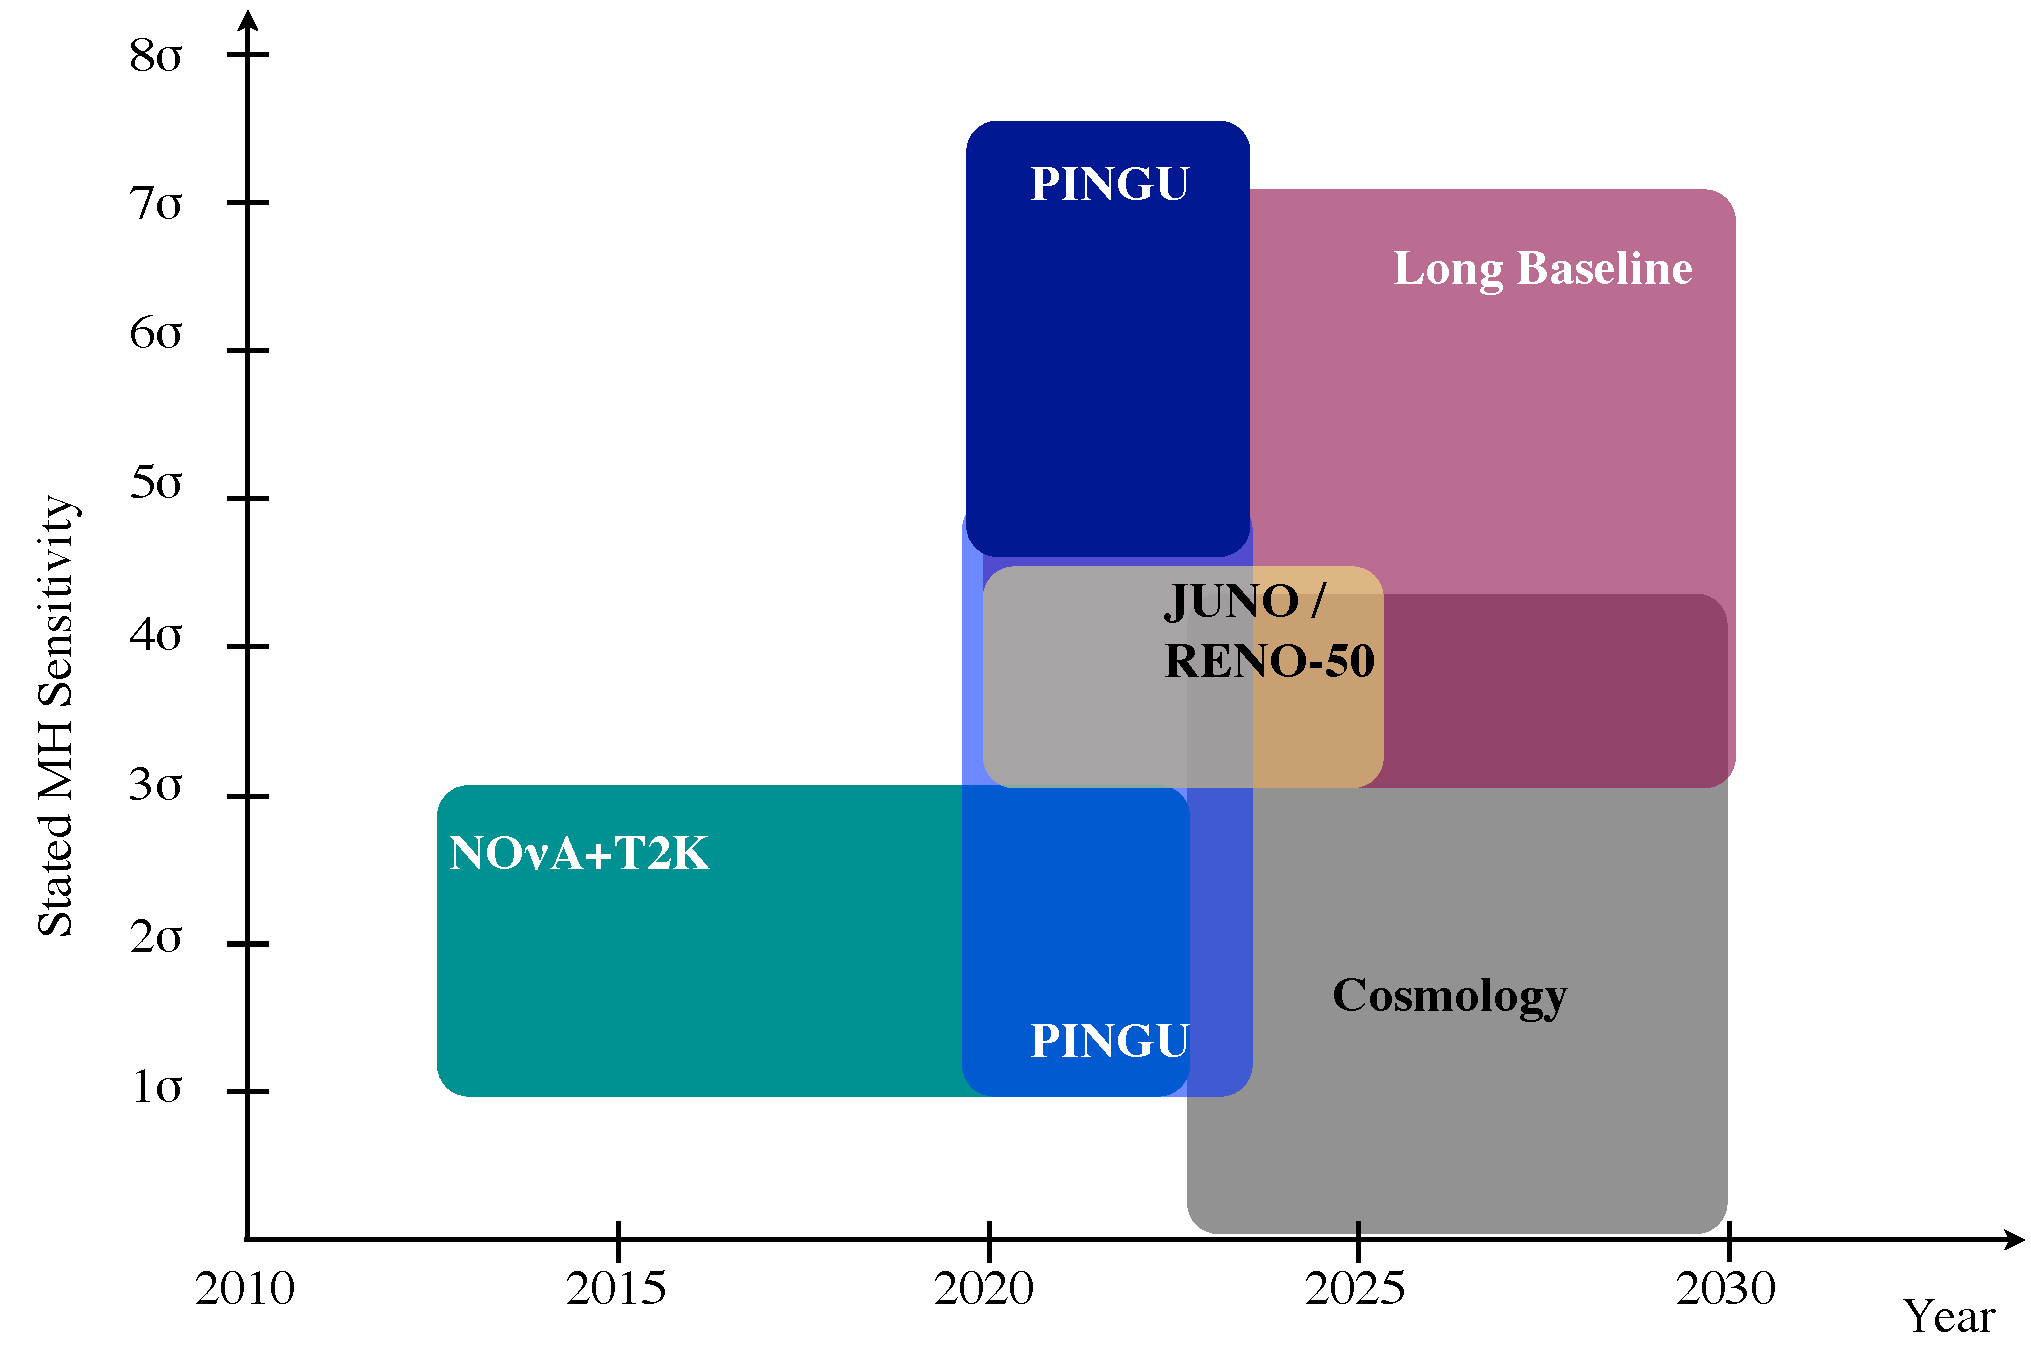
\includegraphics[width=0.95\textwidth]{./finalbubbleplot.pdf}
\caption{ Summary of sensitivities to the neutrino mass hierarchy for various experimental approaches, with timescales, as claimed by the proponents in each case.  In the case of PINGU, for which multiple studies exist, the proponents' stated sensitivity~\cite{atm:pingu} is shown in the dark blue region, with the larger blue region representing the independent analysis of Ref.~\cite{atm:Winter}.  One difference between the two is the consideration of a wider range of oscillation parameters in~\cite{atm:Winter}  (see Section~\ref{s:atm} for details).
% 
%Conclusions from independent studies such as~\cite{atm:Winter} have not been represented in this figure, since equivalent studies are not available for all experiments.  
The vertical scale of each region represents the spread in the expected sensitivity after the full exposure.  We do not attempt to project the natural increase in sensitivity over time. Note: the ``long baseline'' region represents the inclusive range of sensitivities for individual long-baseline experiments (LBNE, HyperK, and LBNO) rather than a combined sensitivity.
\label{f:bubble}}
\end{center}
\end{figure} 

Of the experiments we have considered, only the long-baseline 
experiments (LBNE in combination with T2K/\NOvA, the European-based LBNO, and HyperK's combined long-baseline and atmospheric data) have demonstrated the
ability to measure the mass hierarchy with a statistical significance
of at least $4\sigma$ regardless of the
value of $\delta_{CP}$ and other oscillation parameters. This statement is not without some
caveats. So far, LBNE sensitivities are based on parameterized
(``toy'') simulations, rather than a complete understanding of
the complicated physics involved in neutrino-nucleus interactions at low
energies, or even detailed reconstruction algorithms in LAr
TPC. Addressing these deficiencies is very important. Also, there is a
finite risk that with the long
timescale of LBNE construction (the 10-year run is planned to start in
about 2020), some other experiment(s) will determine the hierarchy
before LBNE produces a result. This would put a costly project in an
unfortunate position to confirm someone else's discovery. 

In addition to LBNE, both Japan and Europe are considering
long-baseline neutrino oscillation experiments. HyperK is a
Megaton-scale water Cherenkov detector, to be constructed in the
Kamioka mine, with the same baseline (about 300 km) from the neutrino
source at J-PARC as T2K. With the short baseline, HyperK needs
atmospheric neutrino data to break the degeneracy between the matter
effects and $\delta_{CP}$, and to determine the mass hierarchy with
a significance of at least $3\sigma$. The timescale and costs for
HyperK are comparable to that of LBNE. 

European long-baseline projects (LAGUNA-LBNO) involve an intense neutrino
source at CERN, a near detector, and a (phased) 
100 kT underground LAr detector at 
Pyh\"asalmi in Finland, at a baseline of 2300~km.  The long
baseline, large detector mass, underground location, near detector,
and a broad-band neutrino beam from a 2~MW proton source make LAGUNA-LBNO
an ultimate neutrino oscillation experiment, with outstanding
sensitivity to both the neutrino mass hierarchy and
$\delta_{CP}$. However, the timescale, costs, and priority to host such
an experiment in Europe are not well defined at present. 

JUNO is a 20~kT liquid scintillator detector to be located at
the solar oscillation maximum, approximately 60~km away from two
nuclear power plants in China. This experiment plans to exploit subtle
distortions in the neutrino energy spectrum sensitive to the sign of
$\Delta m^2_{32}$.  RENO-50 is a similar experiment proposed in South Korea.  
This measurement is extremely challenging, both technologically and in terms of required experimental precision.  
Successful determination of the neutrino mass hierarchy depends
critically on achieving unprecedented energy resolution
and controlling the energy scale systematics to about 1\%. 
%., and knowing the absolute value of $\Delta m^2_{32}$ to 1\%, a level that is unlikely to be
%achieved prior to results from LBNE. 
%At present, we are unable to independently verify how the experiment will achieve the stated systematic requirements. 
If these challenges can be met, then the hierarchy could be measured to $>3\sigma$ ($>4\sigma$) assuming current (future $1.5\%$-level) uncertainties on $\Delta m^2_{32}$.  

Another proposed experiment that could in principle rapidly determine
the neutrino 
mass hierarchy is PINGU, a dense array of phototube strings in the
middle of the IceCube detector at the South Pole. The measurement relies
on polar-angle dependent distortions in the neutrino energy
spectrum due to matter-induced neutrino
oscillations. With the copious samples of upward-going electron and
muon neutrinos and large target mass, PINGU 
has excellent statistical sensitivity to the mass hierarchy.
%could determine the mass hierarchy with a very large significance ($5-6\sigma$) as early as 2022. 
However,
disentangling the hierarchy-dependent effects from the data requires
an excellent energy resolution and understanding the energy scale
systematics in the detector.  The sensitivity also depends on Nature's choice of oscillation parameters, including the hierarchy itself.
As evaluated by the proponents,  the sensitivity of PINGU could be $\sim 4.8$-$7.6\sigma$ with 5 years of data.  
While the potential for a decisive,
inexpensive, and fast measurement is there, we do not feel the
systematic issues have been fully addressed by the proponents to
date. These studies are ongoing as of this writing. 
An independent study finds a larger range of potential sensitivities ($1-5\sigma$), including a lower bound for the case of an inverted hierarchy, which can be partially mitigated by combination with T2K/\NOvA\ data. 

Future dark energy experiments such as MS-DESI (formerly BigBOSS),
Euclid, and LSST, in combination with the Cosmic
Microwave Background measurements, have the capability to measure the
sum of the neutrino masses with a precision relevant to the neutrino
mass hierarchy.  Should the hierarchy 
be normal and the neutrino masses minimal, global cosmological fits
could discern the neutrino mass hierarchy on a timescale comparable
to that of LBNE. Early indication can be obtained from  currently
running or near-future measurements. These measurements
rely on the present best cosmological model ($\Lambda$CDM), which is
supported by the wealth of astrophysical data. 

While any individual measurement in the next decade may be susceptible to large uncertainties, either statistical or systematic, a combination of results from multiple experiments and techniques could yield a greater confidence in a determination of the mass hierarchy.  We have not explicitly considered the potential improvements from such combinations, although independent studies exist~\cite{atm:Winter, combo}.  It is  our hope that several of the experiments here described will be pursued.
  Ultimately, a cross check between multiple techniques will be required for any decisive, unambiguous determination of the mass hierarchy.

\begin{sidewaystable}[!htdp]
\begin{center}
\caption{Comparison of mass hierarchy experiments.  ``NH'' refers to the normal hierarchy. 
In the case of PINGU, for which multiple studies exist, both the sensitivities claimed by the proponents~\cite{atm:pingu} and the independent analysis of Ref.~\cite{atm:Winter} are presented.
\label{t:MH2}}
\begin{tabular}{ m{3cm}p{3cm}p{3.cm}p{6cm}p{0cm}}
\hline \hline
%{\bf Technique} Experiment  & Timescale   & Scope for mass hierarchy & Other scope & Major concerns &LBL opportunities  \\
{\bf Technique} $\qquad$ Experiment  &  \centering{MH sensitivity} & \centering{Timescale for  results}    &  \centering{Major concerns} &   \\
\hline 
\bf Accelerator \\
T2K+\NOvA		&  \centering{1--3$\sigma$}
%Limited. NOvA\cite{Vahle, patterson}: little chance of 3$\sigma$, 25\% chance of 95\% CL at 700kw, 3+3 yrs 		
& \centering{$\sim$2020}		& \centering{Non-optimal baselines} & \\
HyperK 	&   \centering{$>3\sigma$ with atmospheric} 								& \centering{$\sim$2030} 		 &  \centering{Likelihood of going ahead} &   \\
LAGUNA-LBNO 	&   \centering{$>5\sigma$} 								& \centering{$\sim$2025} 		 &  \centering{Likelihood of going ahead} &    \\
 LBNE phase I 	&  \centering{3$\sigma$ (2$\sigma$) over 80\% (100\%) of $\delta_{CP}$}																& \centering{$\sim$2030} 	 	&    \\
 LBNE 34~kT 	&  \centering{$>6\sigma$}																& \centering{$\sim$2030} 	 	& \centering{Assuming Phase-I timescale}  & \\
\hline
\bf Reactor \\
 JUNO 		&  \centering{3--4$\sigma$} 				& \centering{$\sim$2025}  		&  \centering{Energy scale \& resolution} & \\
\hline 
\bf Atmospheric \\
 PINGU 			&  \centering{$4.8-7.6\sigma$~\cite{atm:pingu}  $1-5\sigma$~\cite{atm:Winter} (dependent on oscillation parameters)}
 & \centering{$\sim$2023} 		&  \centering{Energy scale \& resolution, correlated
 parameters} & \\
\hline
\bf Cosmology \\
 All %MS-DESI (BigBOSS), LSST, Euclid, etc. %& Promising {\it iff} it is normal with minimal masses.  
&  \centering{0--4$\sigma$ $\qquad\qquad$(3--4$\sigma$ for NH and minimal masses)}
& \centering{$\sim$2025}   & \centering{Measures sum of masses -- can only determine hierarchy for minimal masses} & \\
\hline \hline
\end{tabular}
\end{center}
\end{sidewaystable}%
